%**************************************************************************
%*
%*  Paper: ``INSTRUCTIONS FOR AUTHORS OF LATEX DOCUMENTS''
%*
%*  Publication: 2016 Winter Simulation Conference Author Kit
%*
%*  Filename: wsc16paper.tex
%*
%*  Date: January 31, 2001   Time:  9:45 PM
%*      BASE of current version: Feb 01, 2010 (primary WSC'10 LaTeX file)
%*
%*  Word Processing System: TeXnicCenter and MiKTeX
%*
%*
%*  All files need the following
\input{wsc16style.tex}     % download from author kit.  Style files for wsc formatting. Don't remove this line - required for generating the final paper!

\documentclass{wscpaperproc}
\usepackage{latexsym}
%\usepackage{caption}
\usepackage{graphicx}
\usepackage{mathptmx}
\usepackage{caption}
\usepackage{subcaption}
\usepackage{pgfplots}
\usetikzlibrary{patterns}
\usepackage{tikz}
\usepackage{multirow}

\usepackage{amsmath}
\usepackage{amsfonts}
\usepackage{amssymb}
\usepackage{amsbsy}
\usepackage{amsthm}
\usepackage{algorithm}
\usepackage{gensymb}
\usepackage[noend]{algpseudocode}
\renewcommand{\algorithmicforall}{\textbf{for each}}



%
%****************************************************************************
% AUTHOR: If you do not wish to use hyperlinks, then just comment
% out the hyperref usepackage commands below.

%% This version of the command is used if you use pdflatex. In this case you
%% cannot use ps or eps files for graphics, but pdf, jpeg, png etc are fine.

\usepackage[pdftex,colorlinks=true,urlcolor=blue,citecolor=black,anchorcolor=black,linkcolor=black]{hyperref}

%% The next versions of the hyperref command are used if you adopt the
%% outdated latex-dvips-ps2pdf route in generating your pdf file. In
%% this case you can use ps or eps files for graphics, but not pdf, jpeg, png etc.
%% However, the final pdf file should embed all fonts required which means that you have to use file
%% formats which can embed fonts. Please note that the final PDF file will not be generated on your computer!
%% If you are using WinEdt or PCTeX, then use the following. If you are using
%% Y&Y TeX then replace "dvips" with "dvipsone"

%%\usepackage[dvips,colorlinks=true,urlcolor=blue,citecolor=black,%
%% anchorcolor=black,linkcolor=black]{hyperref}
%****************************************************************************



		



%
%****************************************************************************
%*
%* AUTHOR: YOUR CALL!  Document-specific macros can come here.
%*
%****************************************************************************

% If you use theoremes
\newtheoremstyle{wsc}% hnamei
{3pt}% hSpace abovei
{3pt}% hSpace belowi
{}% hBody fonti
{}% hIndent amounti1
{\bf}% hTheorem head fontbf
{}% hPunctuation after theorem headi
{.5em}% hSpace after theorem headi2
{}% hTheorem head spec (can be left empty, meaning `normal')i

\theoremstyle{wsc}
\newtheorem{theorem}{Theorem}
\renewcommand{\thetheorem}{ \arabic{theorem}}
\newtheorem{corollary}[theorem]{Corollary}
\renewcommand{\thecorollary}{\arabic{corollary}}
\newtheorem{definition}{Definition}
\renewcommand{\thedefinition}{\arabic{definition}}


%#########################################################
%*
%*  The Document.
%*
\begin{document}

%***************************************************************************
% AUTHOR: AUTHOR NAMES GO HERE
% FORMAT AUTHORS NAMES Like: Author1, Author2 and Author3 (last names)
%
%		You need to change the author listing below!
%               Please list ALL authors using last name only, separate by a comma except
%               for the last author, separate with "and"
%
\WSCpagesetup{Sunderrajan, Viswanathan, Cai and Knoll}

% AUTHOR: Enter the title, all letters in upper case
\title{DATA DRIVEN ADAPTIVE TRAFFIC SIMULATION OF AN EXPRESSWAY}

% AUTHOR: Enter the authors of the article, see end of the example document for further examples
\author{Abhinav Sunderrajan\\ [12pt]
TUM CREATE Ltd \\
1 CREATE Way\\
138602, SINGAPORE\\
% Multiple authors are entered as follows.
% You may also need to adjust the titlevbox size in the preamble - search for titlevboxsize
\and
Vaisagh Viswanathan\\[12pt]
TUM CREATE Ltd \\
1 CREATE Way\\
138602, SINGAPORE\\
\and
Wentong Cai\\ [12pt]
School of Computer Engineering\\
Nanyang Technological University\\
Nanyang Avenue 639798, SINGAPORE\\
\and
Alois Knoll\\ [12pt]
Robotics and Embedded Systems Group \\
Department of Informatics\\
Technische Universit\"at M\"unchen\\
Boltzmannstra{\ss}e 3\\
D-85748 Garching bei M\"unchen, GERMANY
}



\maketitle

\section*{ABSTRACT}
Ubiquitous data from a variety of sources such as smart phones, vehicles equipped with GPS receivers and fixed sensors makes it an exciting time for the implementation of several {\it Advanced Traffic Information and Management Systems} (ATMS). Leveraging this data for current traffic state estimation along with short term predictions of traffic flow can have far reaching implications for the next generation of Intelligent Transportation Services (ITS). In this paper, we present our proof-of-concept of a data driven adaptive traffic simulation for short term prediction and control of traffic flow along a real world expressway through dynamic ramp-metering.

\section{INTRODUCTION}
\label{sec:intro}


A  dynamic data driven adaptive simulation incorporates real-time data from the physical system to initialize or steer the simulation system. {\it Symbiotic Simulation} introduced in~\cite{fujimotoeditors} is a special class of DDDAS involving a mutually beneficial relationship between the physical systems which provides continuous inputs to steer the simulation which in turn gives recommendations to the physical system. The challenges in terms of incorporating real-time data streams to steer executing simulations have been discussed in~\cite{darema2004dynamic}. 

Dynamic data driven simulations have found applications in several domains. An emergency detection and response system by~\shortciteN{schoenharl2006wiper} has been developed by processing call data records in real-time for identifying anomalies and emergencies. Plans for further actions when emergencies are detected are determined by agent based simulations. \cite{celik2013dddams} have been employed multi-agent data driven simulations for reliable and efficient dispatching of electricity under distributed generation for smart grids. Simulation based short-term forecasting using real-time data streams has found applications in modeling and tracking wildfires by~\shortciteN{douglas2006dddas} and ocean state observation and forecasting by~\shortciteN{patrikalakis2004towards}. Considering the wide variety of domains that employ such data driven simulations, it is evident that making use of the information provided by several traffic participants will be beneficial for various ITS based services.

In this paper, we present a symbiotic traffic simulation platform which receives continuous from the physical system i.e. the road network to initialize a predictive faster than real time simulation. Based on the results of the predictive simulations, a recommendation is sent back to the road network for optimizing traffic flow. The physical system is modeled as a high-fidelity agent based microscopic traffic simulation incorporating acceleration and lane change models of the agents. The short-term predictive system which receives traffic state input from the physical system uses a macroscopic traffic model to employ a simulation based optimization strategy. The recommendations of this predictive system are given back to the microscopic simulation (modeling the physical system) and evaluated for efficacy.

The organization of the rest of this paper is as follows. In the next section we discuss the symbiotic traffic simulation framework in greater details. In section~\ref{sec:modelling} discusses the model used to represent the physical system and the model used in the macroscopic prediction and optimization system. The section also covers {\it ramp-metering} which is the control action recommended by the predictive system for traffic flow optimization of a real world expressway. Section~\ref{sec:experiments} discusses the parameters of the microscopic and macroscopic simulations, the environment (road-network) simulated and the calibration of the predictive system. The results of the traffic flow optimization through dynamic ramp-metering is discussed in Section~\ref{sec:results}. We conclude this paper in Section~\ref{sec:conclusion}.



\section{SYMBIOTIC TRAFFIC SIMULATION FRAMEWORK}
\label{sec:methodology}
\begin{figure}[!htbp]
    \centering
    \includegraphics[scale=0.50]{images/methodology.pdf}

    \caption{Symbiotic traffic simulation system.}
    \label{fig:sts-platform}
  \end{figure}

For an accurate representation of the physical world, we employ agent-based microscopic traffic simulations. The agent-based simulations were employed owing to the lack of resources to implement the recommendations of the predictive simulation on a real world road network. The {\it floating car data} (FCD) provided by the microscopic simulation were used to initialize the initial state of the predictive {\it Cell Transmission Model} (CTM)~\cite{daganzo1994cell} based macroscopic simulation. Refer to Figure~\ref{fig:sts-platform} illustrating the symbiotic relationship between the physical and the predictive systems. The predictive system gives  recommendations to the physical system  to optimize traffic flow after running multiple iterations to evaluate different {\it what-if} scenarios. See~\shortciteN{aydt2008preventive} for what-if analyses using symbiotic simulations.

The primary reason for employing a macroscopic simulation for the predictive system  is computational efficiency. A gradient-based optimization strategy involves assessing the fitness of several candidate solutions in parallel. The fitness of a solution is given at the end of a stochastic predictive traffic simulation over a predetermined time horizon.  The above argument motivates us to go in for a cell based macroscopic model despite the relative lack of accuracy in comparison to the microscopic models. The execution time of a CTM based algorithm is proportional to the number of cells simulated (see Algorithm~\ref{algo:ctm}) thus making it an ideal model for a predictive simulation based optimization system.

A microscopic traffic model involves simulating hundreds of thousands of agents and updating their speeds and positions every time-step. Further, modeling lane changes involves acquiring locks (in the context of parallel programming) on multiple lanes making a large scale microscopic simulation computationally expensive (See~\cite{aydt2013multi}). In the subsequent sections we show that our calibrated first-order traffic simulation can model the evolution of traffic state with minimal error (in comparison to the high fidelity microscopic models) provided it is well calibrated and initialized with a reasonably good estimate of the current traffic state in the physical system. 
  
  
 \section{MODELING APPROACH} 
 \label{sec:modelling}
 In this Section we discuss our models that govern the agent based microscopic simulation representative of the physical system and the CTM based faster-than-real-time predictive simulation. 
 
 
\subsection{Modeling of the Physical System}

The agent based traffic simulation representing the physical system is based on the {\it SEMSim} platform~\shortciteN{zehe2015semsim,aydt2013multi}. SEMSim is a high fidelity agent-based microscopic simulation. It uses the {\it Intelligent Driver Model}~(IDM)~\shortciteN{treiber2010open} and MOBIL~\shortciteN{kesting2015general} as the acceleration and lane change models respectively.

The IDM is an accident free model which ensures that a vehicle attains the desired velocity at free flow and maintains the safe bumper to bumper distance to the leading vehicle. It also ensures that the acceleration is an increasing function of the speed and distance to the leading vehicle and a decreasing function of its speed. MOBIL, the lane change model ensures that the resultant accelerations and decelerations for a vehicle and its followers in the old and new lanes does not exceed a safe threshold. A lane change is done only if a vehicle gains speed without violating the safety and inconvenience (to the old and new followers) criteria.


The simulation takes as input a road network detailing the lanes constituting the roads to be simulated. Road segments that don't have a preceding road segment are considered {\it sources} and those without a subsequent segment are {\it sinks}. The traffic thus flows from the sources to the sinks. The route taken by each agent is determined  based on the turn ratios  ranging between $0.0$ and $1.0$ specified at each off-ramp expressway intersection. The details of the probability distributions and other parameters governing this simulation are discussed in Section~\ref{sec:experiments}. Vehicles are generated at each source as a Poisson process with $\epsilon_{s}$ representing the mean number of vehicles generated at each source link $s$. Note that SEMSim and the term physical system shall be used interchangeably over the rest of this paper.


\subsection{Modeling of Predictive System}

The predictive, faster than real time macroscopic simulation is based on the stochastic variant of the Cell transmission model~\shortciteN{boel2006compositional} and METANET~\shortciteN{kotsialos2002traffic}. The cell network, $\mathbb{C}$ is comprised of $n$ cells. At each time instant, $t=k.T$, $k=0,1, .... K$ (where $K$ is the time horizon) the state of all cells are updated. The discrete event time step is denoted by $T_{ctm}$.
  
The state of a cell $c_i\in \mathbb{C}$ at each time step $k.T_{ctm}$ is determined by the concept of {\it sending} $S_i(k)$ and {\it receiving potentials} $R_i(k)$. $S_i(k)$ and $R_i(k)$ represent the number of vehicles cell $c_i$ can send and receive at $k$. The mean and standard deviation of speed for a cell $c_i$ are denoted by $v_i(k)$ and $v_i^{sd}(k)$ respectively.  The number of vehicles in a cell $c_i$ at time-step $k$ is given by $N_{i}(k)$. While $N_i^{max}(k)$ represents the maximum number of vehicles that can be accommodated in cell $c_i$ given an average speed of $v_i(k)$. $N_i^{max}(k)$ is given by
\begin{equation}
\label{eq:nmax}
N_i^{max}(k)=\frac{l_i.\lambda_i}{T_{gap}.v_{i}(k)+ L_{eff}}
\end{equation}
Where $L_{eff}$, the {\it effective} vehicle length represents the sum off mean vehicle length and minimum gap. $T_{gap}$ represents the safe time gap.
The length of cell $c_i$ is denoted by $l_i$ which is variable while being subject to the constraint $l_i \le V_0^i\times T_{ctm}$. Where $V_0^i$ is the constant free-flow speed for the cell. This constraint ensures that no vehicle can enter and exit a cell within one time-step. The number of lanes in cell $c_i$ corresponding to the associated road-link is denoted by $\lambda_i$. The outflow in number of vehicles at time-step $k$ from cell $c_i$ is given by $y_i(k)$ while the density in number of vehicles per unit distance per lane is denoted by $\rho_i(k)$. The {\it critical density} $\rho^{crit}_i$ separating free and congested traffic of a cell $c_i$ is given by 

\begin{equation}
\label{eq:critden}
\rho^{crit}_i=\frac{1}{V_0^i.T_{gap}+L_{eff}}
\end{equation}

Other parameters in this predictive simulation are terms $\kappa, \delta$ and $\phi$. The first two adapt the speed of the vehicles after on-ramp expressway merging while last term $\phi$ adapts the speed of cell where a lane drop occurs. Finally $V^{out}_{min}$ denotes the minimum cell speed of cell when it is completely congested. $V^{out}_{min}$ thus models the fact that some vehicles exit a bottleneck with a minimum speed. 

\subsubsection{Cell network}
\begin{figure}[htb]
    \centering
    \includegraphics[scale=0.55]{images/cellNetwork.pdf}

    \caption{An illustrative cell network.}
    \label{fig:cell-network}
  \end{figure}

The cells constituting the cell network $\mathbb{C}$ are classified into five different types as shown in Figure~\ref{fig:cell-network}. Note that this is an illustrative network and not the real world expressway (see Section~\ref{subsec:pie}) simulated for the experiments. The {\it Merging} cells are associated with the parameter {\it merge priority} $\mu\in [0.0,1.0]$ which controls the proportion of vehicles that moves to the next cell in a given time-step. Correspondingly $\mu^{on}_{ramp}$ and $\mu_{exp}$ are the merge priorities of the on-ramp and expressway cells respectively. The {\it Source} and {\it Sink} cells are not physically related to any of the road links. The source and sink cells are effectively {\it ghost cells}, the former injects agents into the simulation while the agents exit the simulation through the latter. A {\it Diverging} cell is associated with the turn ratios $\tau$ ranging between $0.0$ and $1.0$ representing the proportion of vehicles exiting the expressway through off ramp and those continuing to traverse along the expressway. Cells $C_3$ and $C_9$ are considered {\it predecessors} of cell $C_4$ while cells $C_{10}$ and $C_7$ are considered {\it successors} of cell $C_6$. The creation of vehicles at the source cells are akin to the Poisson process used to create vehicles at the source links as explained in the previous section.

\begin{algorithm}[h]
\caption{CTM based macroscopic predictive simulation.}
\label{algo:ctm}

%$T\sum\limits_{\substack{k=k_1}}^{k=K}N(k)$ 
\begin{algorithmic}[1]

\While{$t<K$}
\ForAll{$c_i \in \mathbb{C}$}
\State update sending and receiving potentials.
\EndFor

\ForAll{$c_i \in \mathbb{C}$}
\State update outflow.
\EndFor

\ForAll{$c_i \in \mathbb{C}$}
\State update number of vehicles.
\State update density.
\EndFor

\ForAll{$c_i \in \mathbb{C}$}
\State update average speed $v_{i}$
\State update the maximum number of vehicles $N^{max}_{i}$
\EndFor

$t=t+k.T_{ctm}$
\EndWhile


\end{algorithmic}
\end{algorithm}

Algorithm~\ref{algo:ctm} shows the progress of the simulation over the prediction time horizon $K$. The equations governing the state of all cells at each time step are provided in the Appendix~\ref{appendix:a}. While the details of the model parameters are discussed in Section~\ref{sec:experiments}.


\subsection{Ramp Metering}
\label{subsec:ramp-metering}
Ramp metering is a traffic control mechanism implemented in several cities across the world to reduce the congestion on expressways~\cite{bogenberger1999advanced}. Ramp meters are traffic signals placed at the intersection of on-ramps and expressways. Ramp meters regulate the flow of vehicles along the ramps so as to minimize the turbulence caused due to merging vehicles disrupting the mainline flow. Care must be taken to ensure that the queue of the vehicles waiting along the on-ramps does not spill into the preceding urban street network. 

Ramp metering strategies are classified into two types, {\it fixed-time} and {\it reactive}~\shortcite{papageorgiou2003review}. The fixed time strategy is based historical data pertaining to flow rates along the on-ramps and the expressway at different times of the day. The main drawback of the fixed time strategy is that their settings are based on historic rather than real time data. It does not take into account the varying nature of traffic demand and the occurrence of events such as accidents and road blocks which could cause massive congestions. 

Reactive ramp metering strategies aim to optimize the flow of traffic based on real-time measurements. Reactive ramp metering is classified into two types {\it Local Ramp Metering} and {\it Multivariable Regulator Strategies}~\shortcite{papageorgiou2003review}.  The former makes use of measurements in the vicinity of an on-ramp to regulate the flow on the ramp. The control strategy applied for an on-ramp is independent of the measurements and controls applied in other on-ramps in the vicinity. While the latter makes use of the system wide measurements to simultaneously regulate traffic flow along all on-ramps. See~\cite{bogenberger1999advanced} for a review on several implemented and proposed ramp metering strategies.

In this paper we employ a simulation based optimization strategy to develop a solution for a system wide ramp metering strategy of a real world expressway by regulating the flow on all on-ramps simultaneously. A control mechanism tries to minimize the total number of vehicles $N_{total}$ in the system over a given time horizon $K$(~\shortcite{papageorgiou2003review}) as shown in Equation~\ref{eq:minimize}

\begin{equation}
\label{eq:minimize}
N_{total}=T.\sum\limits_{\substack{k=0}}^{k=K}N(k)
\end{equation}
where $N(k)$ is the number of vehicles at time step $k$. $T$ represents the simulation time-step.


The system-wide ramp controller designed for this paper determines the maximum allowable {\it queue-percentage} $q^{th}_r$ (Equation~\ref{eq:constraint}) for a ramp $r\in \mathbb{R}^{on}_{ramps}$ before turning the phase of the signal to green from red.  $\mathbb{R}^{on}_{ramps}$ is the set of controllable on-ramps in the system.

 \begin{equation}
 \label{eq:constraint}
\frac{N_r(k)}{N^{max}_r(k)}\le q^{th}_r
 \end{equation}
 Where $N_r(k)$ and $N^{max}_r(k)$ is the number and the maximum number of vehicles on the on-ramp $r$ at time step $k$. $N^{max}_r(k)$ at time-step $k$is determined from Equation~\ref{eq:nmax}. Concretely the task is to find the ideal value of $q^{th}_r$ for all on-ramps so as to minimize $N_{total}$.


\section{EXPERIMENTS}
\label{sec:experiments}


\subsection{The Simulated Environment}
\label{subsec:pie}

\begin{figure}[!htbp]
    \centering
    \includegraphics[scale=0.40]{images/PIE.jpg}

    \caption{Simulated section of P.I.E (Singapore) and location of all on/off ramps.}
    \label{fig:pie-changi}
  \end{figure}

\begin{table}[htb]
 \centering
 \caption{Location of all On/Off ramps along the expressway.}
\begin{tabular}[b]{ccc}\hline
      {\bf DISTANCE} (m) & {\bf RAMP TYPE} \\ \hline
     583.98 & On-Ramp \\ 
     1973.35 & Off-Ramp \\ 
     2489.87 & On-Ramp \\ 
     3261.27 & Off Ramp \\ 
     4071.9 & On-Ramp \\ 
     4834.84 & Off-Ramp \\ 
     5531.18 & On-Ramp \\ 
     5743.11 & Off-Ramp \\ 
     5965.29 & On-Ramp \\ 
     6207.74 & Off-Ramp \\ \hline
     \end{tabular}
     \quad
     \begin{tabular}[b]{ccc}\hline
       {\bf DISTANCE} (m) & {\bf RAMP TYPE} \\ \hline
     7025.15 & On-Ramp \\ 
     7658.4 & On-Ramp \\ 
     8040.83 & Off-Ramp \\ 
     8554.28 & On-Ramp \\ 
     8807.94 & Off-Ramp\\ 
     9591.84 & On-Ramp \\ 
     10148.24 & Off-Ramp \\ 
     11286.2 & On-Ramp \\ 
     11637.04 & On-Ramp \\ 
     12438.23 & Off-Ramp \\  \hline
    \end{tabular}
      \label{table:on-off-ramp}
\end{table}

For the experiments in this paper, we simulated a $13$ km stretch of P.I.E (Pan Island Expressway) in central Singapore (Figure~\ref{fig:pie-changi}) with all on and off ramps. The on-ramps and the first P.I.E link are sources, while all off ramps and the last link on P.I.E are sinks. Refer to the Table~\ref{fig:pie-changi} for the location of all on/off ramps (or {\it static bottlenecks}) starting from the beginning of the first road-segment on P.I.E. The average distance between two bottlenecks is around $565$ m along this stretch of P.I.E. The turn ratios for all off-ramps is kept constant at $0.25$. This implies that $25\%$ of all vehicles exit at a given off ramp while the remaining $75\%$ of the vehicles continue to travel on the main expressway. The number of lanes in the simulated stretch of the expressway varies between $3$ and $6$.



\subsection{Parameters of the Microscopic Simulation}

\begin{table}[!htbp]
\centering
\caption{The microscopic simulation parameters}
\begin{tabular}{ccc}\hline
\textbf{\begin{tabular}[c]{@{}c@{}}Simulation\\ parameter\end{tabular}} & \textbf{Description}                                                                               & \textbf{Range}                                                                                \\ \hline \\
$T_{semsim}$                                                                 & \begin{tabular}[c]{@{}c@{}}Simulation time step.\end{tabular} & $250$ milliseconds                                                                                       \\
$s_{0}$                                                                 & \begin{tabular}[c]{@{}c@{}}Minimum bumper-to-bumper distance \\ to the front vehicle.\end{tabular} & $2.0$ m                                                                                       \\
$T_{gap}$                                                                       & Time gap to preceding agent                                                                        & $1.4$ sec                                                                                     \\
$l$                                                                       & Agent/vehicle length                                                                  & \begin{tabular}[c]{@{}c@{}}Normal distribution with \\ mean $3.0$ m and standard deviation $0.1$ m\end{tabular} \\
$V_{0}$                                                                 & Desired speed of agent                                                                            & $20$ m/s                                                                                      \\
a                                                                       & Maximum acceleration term for IDM                                                                  & \begin{tabular}[c]{@{}c@{}}Uniform distribution between \\ $1.2$ and $1.6~m/s^2$\end{tabular} \\
b                                                                       & Maximum deceleration term for IDM                                                                 & \begin{tabular}[c]{@{}c@{}}Uniform distribution between \\ $1.8$ and $2.2~m/s^2$\end{tabular} \\
$p_{0}$                                                                 & Politeness factor for MOBIL                                                                       & 0.3                                                                                           \\
$\Delta a_{th}$                                                         & Lane change threshold for MOBIL                                                                   & $0.3 ~m/s^2$                                                                        \\ \hline          
\end{tabular}

\label{table:semsim-param}
\end{table}

The microscopic agent based traffic simulation was initialized with the parameters listed in Table~\ref{table:semsim-param}. Parameters such as $a$, $b$ and $l$ are modeled as distributions to take into account heterogeneous driving behaviors and vehicle classes respectively. All of the $11$ on-ramps listed in Table~\ref{table:on-off-ramp} are controllable and regulate the flow of vehicles into the expressway.


\subsection{Calibration of Predictive Simulation}

To ensure that the state predicted by the macroscopic simulation accurately represents the state of the physical system, the model parameters have to be calibrated. We need to identify (and tune) the parameters which will have significant impact in terms of bridging the difference in the state of the physical system and that of the predictive simulation at the end of a given time horizon.

Towards this end we simulated SEMSim representing the physical system over a time horizon $K=2000$ seconds. The mean inter-arrival times of all source links $\epsilon_s$ were kept constant during the time period of the simulation. There are no vehicles in the simulation at times-step $0$. $N_i^{semsim}(K)$ denotes the number of vehicles in each cell of the mainline expressway (corresponding to the cell-network associated with the predictive system) is computed at the end of the microscopic agent-based simulation. 

The task is to identify and then tuning the parameters which influences the predictive simulation resulting in a traffic state so as to minimize the quantity $LSE$ given by
\begin{equation}
LSE=\sqrt{\sum\limits_{i=1}^{i=n_{exp}}(N_i^{semsim}(K)-N_i^{ctm}(K))^2}
\end{equation}
$N_i^{ctm}(K)$ denotes the number of vehicles in each cell of the mainline expressway computed at the end of the predictive simulation time horizon $K$. $LSE$ represents the least square difference between the number of vehicles for all expressway cells (numbering $n_{exp}$) at $K$. The initial state (of zero vehicles at time-step $0$) and the mean inter-arrival times of vehicles for all source cells are the same as that of SEMSim.

\begin{figure}[!htbp]
    \centering
    \includegraphics[scale=0.50]{images/tuning-parameters-ctm.pdf}

    \caption{Polynomial regression to determine the most important parameters for calibrating predictive simulation.}
    \label{fig:var-important}
  \end{figure}

To identify and quantify the parameters which help reduce the difference between the predictive and physical systems, we ran $1600$ iterations of the predictive simulation to the return the least square error $LSE$. The parameters of the CTM based predictive simulation which were varied for each of the iterations are as follows:
\begin{itemize}
\item $\mu^{on}_{ramp}$ uniformly between $0.1$ and $0.6$.
\item $\mu_{pie}$ uniformly between $0.8$ and $1.0$.
\item $V_{min}^{out}$ between $2.0$ m/s  and $6.0$ m/s. 
\item $\phi$ between $1.8$ and $3.6$.
\item $\delta$ between $0.02$ and $0.6$.
\item $T_{gap}$ between $1.2$ sec and $1.5$ sec.
\item $A_m$ between $1.0$ and $4.0$.
\end{itemize}

The results of the linear (polynomial) regression is shown in Equation~\ref{eq:regression}. The $R^2$ Statistic (a measure of model fit indicating the percentage of variance explained by the model) for this model is $0.817$. This model (Figure~\ref{fig:var-important}) clearly shows that the two dominant terms are $T_{gap}$ and $\mu^{on}_{ramp}$. There is a strong interaction term between the two parameters as well as a nonlinearity indicated by the polynomial terms. The model parameters were determined using {\it backward selection} and verified by {\it anova} function. See~\shortciteN{james2013introduction} for an introduction on regression and the terms discussed in this section.
\begin{equation}
\label{eq:regression}
LSE=\beta_0-\beta_1.\mu^{on}_{ramp}+\beta_2.T_{gap}+\beta_3.T_{gap}^2+\beta_4.T_{gap}.\mu^{on}_{ramp}
\end{equation}

Note that $V_{min}^{out}$ is set to $0.0$ for on-ramps at intersection where vehicles come to a complete standstill.

\subsection{Parameters of the Predictive Macroscopic Simulation}

\begin{table}[!htbp]
\centering
\caption{The predictive simulation parameters}
\label{my-label}
\begin{tabular}{ccc}\hline
\textbf{\begin{tabular}[c]{@{}c@{}}Simulation \\ parameter\end{tabular}} & \textbf{Description}                                                                     & \textbf{Value} \\
\hline \\
$\mu^{on}_{ramp}$                                                             & \begin{tabular}[c]{@{}c@{}}Merge priority for on-ramp \\ merging cells\end{tabular}      & 0.22           \\
$\mu_{exp}$                                                              & \begin{tabular}[c]{@{}c@{}}Merge priority for express way \\ merging cells.\end{tabular} & 0.95           \\
$\tau^{off}_{ramp}$                                                             & \begin{tabular}[c]{@{}c@{}}Turn ratio for off ramp\end{tabular}      & 0.25           \\
$\tau_{exp}$                                                              & \begin{tabular}[c]{@{}c@{}}Turn ratio for expressway.\end{tabular} & 0.75           \\
$T_{gap}$                                                                & Safe time gap for vehicles                                                               & 1.25 seconds   \\
$T_{ctm}$                                                                & Simulation time step                                                                     & 2.0 seconds    \\
$V^{out}_{min}$                                                          & Minimum speed in a cell                                                                  & 2.5 m/s        \\
$\kappa$                                                                 & On-ramp merge term                                                                       & 0.45           \\
$\delta$                                                                 & On-ramp merge term                                                                       & 0.27           \\
$V^{out}_{min}$                                                                 & Minimum cell speed                                                                       & 2.50           \\
$A_{m}$                                                                 & Model term                                                                       & 2.34           \\
$\phi$                                                                   & Lane drop term                                                                           & 2.7           
\\ \hline
\end{tabular}
\label{table:ctm-param}
\end{table}


Based on the results of the calibration, the CTM based predictive simulation was initialized with the parameters shown in Table~\ref{table:ctm-param}. The turn ratios at the off-ramp ($\tau_{ramp}^{off}$) and expressway ($\tau_{exp}$) intersections are the same as that of SEMSim (physical system). The mean inter-arrival times $\epsilon_{s}$ for vehicle arrivals at the source cells are also the same as that of the source links in SEMSim. The values of the parameters $A_m, \phi, \kappa$ and $\delta$ are chosen based on the calibration experiments by ~\shortciteN{kotsialos2002traffic}.

\subsection{Traffic Scenario}

Before implementing an optimal ramp metering strategy in the next Section, we discuss the traffic scenario simulated for the physical and predictive systems in brief. The traffic state of the expressway at the end of a time horizon is determined by the inter-arrival time $\epsilon_s$ for all source links and cells. The section of the expressway simulated (Table~\ref{table:on-off-ramp}) consisting of $11$ on-ramps along with the first expressway link has $12$ source links. Table~\ref{table:iat} list the mean inter-arrival times for all source links/cells. Notice that the flow of vehicles into the expressway along all on-ramps  are significantly less (1000 vehicles/hour) except for the ones at $583$ m, $7025$ m and $7658$ m. The system thus needs to find an optimal ramp metering strategy which balances the flow along all on-ramps so as to minimize the surge of vehicles along the three ramps with relatively higher inflow of vehicles.
\begin{table}[!htbp]
\caption{Mean inter-arrival times at all source links/cells}
\begin{tabular}[b]{ccc}\hline
      {\bf DISTANCE} (m) & {\bf RAMP TYPE} & {\bf $\epsilon_s$} (sec)\\ \hline
     0.0 & First P.I.E link & 1.0\\
     583.98 & On-Ramp & 2.0\\ 
     2489.87 & On-Ramp & 3.6\\ 
     4071.9 & On-Ramp & 3.6\\ 
     5531.18 & On-Ramp & 3.6\\ 
     5965.29 & On-Ramp & 2.6\\ \hline
     \end{tabular}
     \quad
     \begin{tabular}[b]{ccc}\hline
       {\bf DISTANCE} (m) & {\bf RAMP TYPE}& {\bf $\epsilon_s$} (sec) \\ \hline
     7025.15 & On-Ramp & 2.0\\ 
     7658.4 & On-Ramp & 2.0\\ 
     8554.28 & On-Ramp & 3.6\\ 
     9591.84 & On-Ramp & 3.6\\ 
     11286.2 & On-Ramp & 3.6\\ 
     11637.04 & On-Ramp & 3.6\\ \hline
    \end{tabular}
      \label{table:iat}
\end{table}


\section{RESULTS}
\label{sec:results}



In this section we quantify the efficacy of using ramp-metering in the physical system (SEMSim) based on the recommendations given by the predictive simulation. As discussed in Section~\ref{subsec:ramp-metering}, we need to find the optimal value of $q^{th}_r \in (0.0,0.8)$ for each of the $11$ on-ramps for the environment simulated. Note that the maximum value of the queue percentage $Q^{th}_{max}$ is set to $0.8$. Thus the controller sets the phase to green when $q^{th}_r$ exceeds $Q^{th}_{max}$ serving as the first constraint.

The two other constraints are:
\begin{enumerate}
\item The minimum phase time for both the red and green phases are $10$ seconds.
\item The signal at an on-ramp can be continuously red only for a maximum of $120$ seconds. After a $120$ second red phase, there is a mandatory green phase for $20$ seconds.
\end{enumerate}
\begin{algorithm}[!b]
\caption{Genetic algorithm for Ramp metering}
\label{algo:ramp-metering}
{\bf Input: }
\begin{itemize}
\item $popsize$, $maxiter$ population size and maximum iterations for GA respectively.
\item $\mathbb{P}\leftarrow \varnothing$, the population.
\item $\mathbb{R}$ the set of controllable on-ramps.
\item $Q^{th}_{max}=0.8$ the maximum allowable queue percentage for any ramp $r\in \mathbb{R}$.
\item $K$ the simulation time horizon for determining the total number of vehicles $N_{total}$.
\item $seed$ the simulation seed for the stochastic simulations.
\end{itemize}
{\bf Result: }Optimal $q_r^{th}$ for each ramp $r \in \mathbb{R}$.
\begin{algorithmic}[1]

\For{$popsize$ times}
	\State $\mathbb{Q}\leftarrow~\varnothing$
	\ForAll{$r \in \mathbb{R}$}
	\State $q_r^{th} \leftarrow randomDouble(q^{th}_{max})$
	\State $\mathbb{Q}\leftarrow~\mathbb{Q} \bigcup q_r^{th}$
	\EndFor
	\State $\mathbb{P} \leftarrow~\mathbb{P}\bigcup \mathbb{Q}$
\EndFor	

\State $Best\leftarrow\varnothing$

\Repeat

$seed\leftarrow randomInt()$
\ForAll{$P_i\in\mathbb{P}$}
\State  $N^i_{total}=SimulateFitness(P_i,~seed)$
\If{$Best==\varnothing$ {\it or} $N^i_{total}<SimulateFitness(Best,~seed)$}
\State $Best\leftarrow P_i$
\EndIf
\EndFor

\State$\mathbb{Z}\leftarrow~\varnothing$
\State $iter\leftarrow0$

\For{$popsize/2$ {\it times}}
	\State {\it Parent} $P_a\leftarrow$ $SelectWithReplacement(\mathbb{P})$
	\State {\it Parent} $P_b\leftarrow$ $SelectWithReplacement(\mathbb{P})$
	\State {\it Children} $C_a, C_b\leftarrow$ $CrossOver(P_a,P_b)$
	\State {$\mathbb{Z}\leftarrow~\mathbb{Z}\bigcup~\{Mutate(C_a),Mutate(C_a)\}$}
\EndFor
\State $\mathbb{P}\leftarrow\mathbb{Z}$
\State $iter\leftarrow iter+1$
\Until{$iter<maxiter$}
\State \Return $Best$
\end{algorithmic}
\end{algorithm}

The first of the above constraint ensures that the phase changes do not thrash around. This gives adequate reaction times for drivers to slow down and accelerate at an intersection. The second constraint ensures that none of the vehicles wait at an on-ramp for an inordinately long time thus preventing the starvation of an on-ramp $r$ even if the $q^{th}_r$ is not exceeded.

We implemented a {\it genetic algorithm GA}~\cite{weise2009global} (See Algorithm~\ref{algo:ramp-metering}) for determining the optimal $q_r^{th}$ for all the controllable on-ramps $\mathbb{R}$. The number of iterations was restricted to $50$ and the population size evaluated was $20$. We used an adaptive {\it Gaussian} mutation which decreases the probability of mutation as the number of iterations increases from $0$ to $maxiter$. $SimulateFitness()$ computes the total number of vehicles $N_{total}$ over a time horizon of $K=1800$ seconds using the CTM based predictive simulation. The GA tries to minimize $N_{total}$ for all individuals over $maxiter$ iterations by varying $q_r^{th}$ between the bounds of $0.0$ and $0.8$ rounded to two decimal places. The best configuration $Best$ of $q_r^{th}$ over all $r \in R$ is returned at the end of the algorithm. Given that the predictive CTM based simulation is stochastic, the {\it seed} of the simulations are changed after every iteration.

The best ramp-meter configuration (determined using the predictive simulation) is now given as a recommendation to the physical system modeled using SEMSim to return the corresponding $N_{total}$ over the same time horizon $K$. Note that the ramp-metering with same constraints pertaining to phase timings are implemented in SEMSim as well. In the next section we determine percentage improvement (in terms of $N_{total}$) in optimizing traffic flow (over the no ramp metering case) when the recommendation of the predictive system is fed back to the simulation system.

\subsection{Efficacy of Ramp Metering}
\begin{figure}[!htbp]
      \centering
      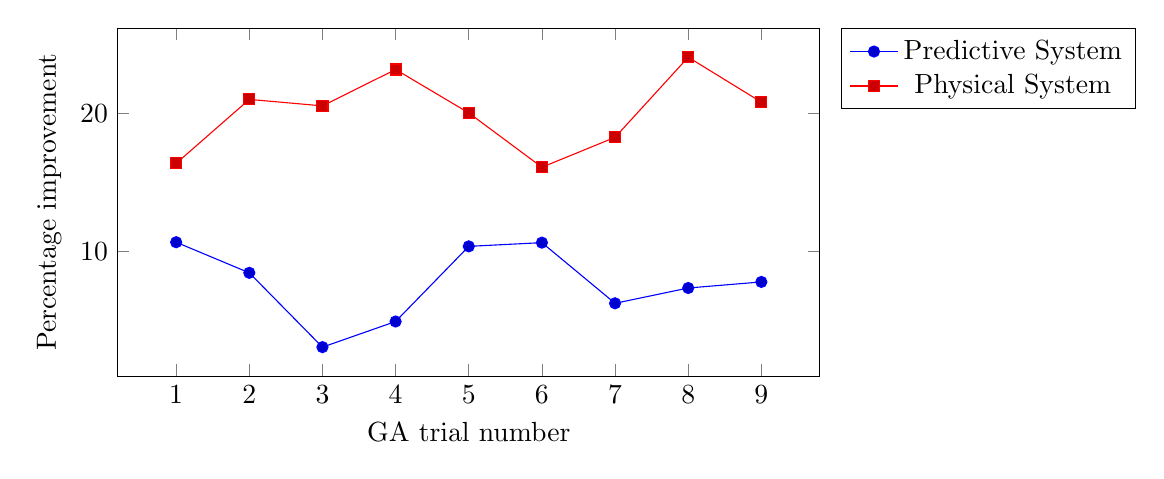
\begin{tikzpicture}
      \begin{axis}[width=10.5cm,height=6.0cm,
      	xlabel={GA trial number},
      	ylabel={Percentage improvement},
      	legend pos=outer north east
      ]
      \addplot coordinates {
      	(1,10.65)    (2,8.43)   (3,3.04)
      	(4,4.9)  (5,10.35)  (6,10.62)  (7,6.22)  (8,7.33)  (9,7.77)	
      };
      
      \addplot coordinates {
            	(1,16.37)    (2,21.01)   (3,20.54)
            	(4,23.18)  (5,20.03)  (6,16.09)  (7,18.26)  (8,24.07)  (9,20.81)	
            };
      \legend{Predictive System, Physical System}
      \end{axis}
      \end{tikzpicture}
      \caption{Percentage improvement of $N_{total}$ over the no ramp metering case.}
      \label{fig:improvement-ramp-metering}
      \end{figure}


Figure~\ref{fig:improvement-ramp-metering} shows the percentage improvement (over the no ramp-metering case) of the metric $N_{total}$ for both predictive system and when its recommendations are fed back into the physical system. $9$ different runs of the GA employing the predictive CTM based simulation return a ramp metering configuration $q_r^{th}$ for all $r\in \mathbb{R}$. This ramp metering configuration is fed back to SEMSim (physical system) to compute the percentage improvement of $N_{total}$ over the no ramp-metering case. The simulation seeds for SEMSim, for all of the $10$ runs (including the no ramp metering case) are varied to account for the stochasticity.
We see clear improvements in the range of $18\%$ to $25\%$ in the physical system even exceeding the percentage improvement predicted by the GA based predictive simulations. The results unequivocally show the benefits of symbiotic traffic simulation provided that the predictive system is calibrated and has sufficient information pertaining to the traffic state in the physical system. 



As a final note, a data driven adaptive simulation and prediction framework for traffic systems should work under reasonable time constraints for predicting short term evolution of state and giving back recommendations to optimize traffic flow. The simulations employed by the predictive system should thus be reasonably fast. The CTM based simulation used by the GA for fitness assessment finished one run over a time horizon of $1800$ seconds in around $250$ milliseconds. The CTM simulation was coded in Java SE 7 and measured in a 2.5GHz Intel i5 system running on Windows 7. Given that it is trivial to parallelize the fitness assessment of all individuals over all the iterations in GA, the methodology detailed in this paper (for ramp metering) can satisfy the soft real-time constraints for traffic flow management.



\section{CONCLUSIONS AND FUTURE WORK}
\label{sec:conclusion}
In this work we have established that data driven predictive simulations can be beneficial towards optimizing traffic flow.  The prediction and optimization system should receive fairly accurate and continuous information on the current traffic state. This information is used for initialization, calibration and steering of the predictive simulations. Accurate current state estimation in turn increases the accuracy of the short term predictions (of evolution of traffic flow) thereby increasing the accuracy of the suggested control measures. Data from traditional fixed sensors can be augmented with FCD from smart phones and vehicle fleets such as taxis and public buses for enhanced traffic state reconstruction. 

Symbiotic traffic simulations offer exiting opportunities to implement and optimize several techniques for traffic flow optimization (other than ramp-metering discussed in this paper) such as adaptive speed limits and dynamic routing. Mobile applications and in car navigation systems provide a great means to disperse information to the traffic participants while the control system receives user anonymized data about vehicle speed, location and even origin-destination flows. This form of a symbiotic simulation based traffic prediction and optimization framework focusing on dispersing and receiving updates from individual drivers will be focus of our future research.

\section*{ACKNOWLEDGMENTS}
This work was financially supported by the Singapore National Research Foundation under its Campus for Research Excellence And Technological Enterprise (CREATE) programme.
\appendix

\section{APPENDIX. EQUATIONS FOR UPDATING CELL STATE}
\label{appendix:a}

\textbf{Updating Sending and Receiving Potentials for all $c_i\in \mathbb{C}$}\\
\begin{subequations} 
\label{eq:sp-rp}
\begin{eqnarray}
term_1=\frac{N_i(k).v_i(k).T_{ctm}}{l_i}\\
term_2=\frac{N_i(k).V^{out}_{min}.T_{ctm}}{l_i}\\
S_i(k+1)= min(max(term_1,~term_2),~N_i(k))\\
R_i(k+1)=N_i^{max}(k)-N_i(k)
\end{eqnarray}
\end{subequations}


\textbf{Updating the outflow for all $c_i\in \mathbb{C}$}\\
 The outflow of an Ordinary cell is given by,
 \begin{equation}
 y_i(k+1)=min(S_i(k+1),~R_{i+1}(k+1))
 \end{equation}
The outflow of a Diverging cell is given by,
 \begin{subequations} 
 \label{eq:diverging-outflow}
 \begin{eqnarray}
 y_{ramp}^{off}(k+1)=min(\tau_{ramp}^{off}.S_i(k+1),~R_{i+1}^{ramp}(k+1))\\
 y_{exp}(k+1)=min(\tau_{exp}.S_i(k+1),~R_{i+1}^{exp}(k+1))\\
 y_i(k+1)=y_{ramp}^{off}(k+1)+y_{exp}(k+1)
 \end{eqnarray}
 \end{subequations}
where $R_{i+1}^{ramp}(k)$ and $R_{i+1}^{exp}(k)$ represent the receive potential of the succeeding Ordinary cells on the off-ramp and expressway respectively. While  $\tau_{exp}$ and $\tau_{ramp}^{off}$ represents the turn ratios for the expressway and the off-ramp  respectively.

The outflow of a Merging cell is given by,\\
if $R_{i+1}(k+1)>S_i(k+1)+S_i^{other}(k+1)$ then,
\begin{subequations} 
 \label{eq:merging-outflow}
 \begin{eqnarray}
 term_1=\frac{\mu.R_{i+1}(k+1)}{\mu+\mu^{other}}\\
 y_i(k+1)=min(term_1,~S_i(k+1))
 \end{eqnarray}
 \end{subequations}
 else,
\begin{equation}
 y_i(k+1)=min(S_i(k+1),~R_{i+1}(k+1).\mu)
 \end{equation}

Where $\mu^{other}$ and $S_i^{other}(k+1)$ represents the merge-priority and the sending potential of the other associated merging cell.

The outflow of a Source cell is given by,\\
\begin{equation}
y_i(k+1)=min(randomPois(\epsilon),~R_{i+1}(k+1))
\end{equation}

where $randomPois(\epsilon)$ represents the random Poisson number with a mean corresponding to the average inter-arrival time ($\epsilon$) for the source link. Note that Sink cell does not have any outflow.\\
Note that the outflow of a ramp cell is set to $0$ when the signal phase is red.\\

\textbf{Update number of vehicles in all cells}\\
\begin{equation}
N_i(k+1)=N_i(k)-y_i(k+1)+\sum\limits_{j=1}^{j=p}y_j(k+1)
\end{equation}
Where $\sum\limits_{j=0}^{j=n}y_j(k)$ represents the total inflow from all of the $p$ predecessors to this cell $i$ where $p$ is either $1$ or $2$.


\textbf{Update density and anticipated density for all $c_i\in \mathbb{C}$}\\
\begin{subequations}
 \label{eq:cell-density}
 \begin{eqnarray}
\rho_i(k+1)=\frac{N_i(k+1)}{l_i.\lambda_i}\\
\rho_i^{antic}(k+1)=\alpha.\rho_i(k)+(1-\alpha).\sum\limits_{j=1}^{j=s}\rho_j(k+1)
\end{eqnarray}
\end{subequations}

Where $\rho_i^{antic}(k+1)$ is the anticipated density which represents the weighted average of the density in the current cell and those of its $s$ successor cells. The coefficient $\alpha\in[0,1]$, we chose $\alpha$ to be $0.85$ thus giving more importance to the density in the current cell while not completely ignoring the speed adaptation resulting from the successor cell densities.


\textbf{Update Average speed and $N_{i}^{max}$ for all $c_i\in \mathbb{C}$}\\


 \begin{equation}
v_i^{temp}(k+1)=
\begin{cases}
\sum\limits_{j=1}^{j=p}[v_{j}(k).y_{j}(k)]+v_i(k)(N_i(k)-y_i(k)), & \text{if } N_i(k+1)\ne 0\\
V_0, & \text{otherwise}
\end{cases}
\end{equation}

\begin{subequations}

\begin{eqnarray}
\label{eq:cell-min}
v_i^{temp}(k+1)=max(v_i^{temp}(k+1),~V^{out}_{min})\\
\label{eq:cell-speed}
v_i(k+1)=\beta_i.v_i^{temp}(k+1)+(1-\beta_i).V_0^i.exp\bigg[\frac{-1}{A_m}\bigg( \frac{\rho_i^{antic}(k+1)}{\rho_i^{crit}}\bigg)^{A_m} \bigg]+\eta_i^{sd}\\
\text{where, }\beta_i=
\begin{cases}
0.8, & \text{if } |\rho_{i+1}^{antic}(k+1)-\rho_i^{antic}(k+1)| \ge 1.0\\
0.2, & \text{otherwise}
\end{cases}
\end{eqnarray}
\end{subequations}

The lane drop term for the merging cell when vehicles merge at the expressway at the end of an on-ramp.
\begin{equation}
\label{eq:lane-drop-term}
v_i(k+1)=v_i(k+1)-\frac{\phi.T_{gap}.\rho_i(k+1).v_i(k+1)^2}{l_i.\lambda_i.\rho_i^{crit}}
\end{equation} 

The speed adaptation at the ordinary cell following the merge cells of the expressway and the corresponding on-ramp. See cell $C_4$ for reference in Figure~\ref{fig:cell-network}.

\begin{equation}
\label{eq:ramp-merge-term}
v_i(k+1)=v_i(k+1)-\frac{\delta.T_{gap}.y^{on}_{ramp}(k+1).v_i(k+1)}{\lambda_i.l_i(\rho_i(k+1)+\kappa)}
\end{equation}
Where $y^{on}_{ramp}(k+1)$ represents the outflow of an on-ramp cell.

 
Equation~\ref{eq:cell-min} ensures that the minimum speed of the cell does not fall below $V^{out}_{min}$, i.e. the minimum speed with which downstream vehicles exit congested zones. Equation~\ref{eq:cell-speed} gives greater weight to the anticipated density term (controlled by the parameter $\beta_i$) if the absolute difference in the density of the current and the successor cells is large. $\eta_i^{sd}$ is the random Gaussian noise term with mean $0$ and standard deviation $v_i^{sd}$. As noted before $v_i^{sd}$ is an input from the physical system.


% Please don't exchange the bibliographystyle style
\bibliographystyle{wsc}
% AUTHOR: Include your bib file here
\bibliography{demobib}

\section*{AUTHOR BIOGRAPHIES}

\noindent {\bf ABHINAV SUNDERRAJAN} works as a Research associate for the "Modeling and Optimization of Architectures and Infrastructure" group at TUM CREATE. He obtained his Bachelors in Electronics and Communication engineering from VTU, India in 2009 and Masters in Computing from NUS, Singapore in 2013. He is curretly pursuing his PhD from the Informatics department in the Technische Universit\"at M\"unchen. His current research interests lie in dynamic data driven applications, simulation based optimization and agent based models for complex systems. His email address is \email{abhinav.sunderrajan@tum-create.edu.sg}.\\

\noindent {\bf VAISAGH VISWANATHAN} obtained his B.Eng degree in Computer Engineering and completed his Ph.D. on "Modeling Behavior in Agent Based Simulations of Crowd Egress" from Nanyang Technological University, Singapore in 2010 and 2015 respectively. He is currently a Postdoctoral Research Fellow at TUM CREATE working on modeling and optimization of architectures and infrastructure. His current research investigates the infrastructure requirements and the environmental impact of large scale electro-mobility from a complex systems perspective. His research interests are primarily agent based modeling and simulation, complex adaptive systems and serious games. His email address is \email{vaisagh.viswanathan@tum-create.edu.sg}.\\

\noindent {\bf WENTONG CAI} is a Professor in the School of Computer Engineering at Nanyang Technological University, Singapore. He is also the Director of the Parallel and Distributed Computing Centre. His expertise is mainly in the areas of Modeling and Simulation (particularly, modeling and simulation of large-scale complex systems, and system support for distributed simulation and virtual environments) and Parallel and Distributed Computing (particularly, Cloud, Grid and Cluster computing). His web page is \hyperref{http://www.ntu.edu.sg/home/aswtcai/}{}{}{http://www.ntu.edu.sg/home/aswtcai/} and his email address is \email{aswtcai@ntu.edu.sg}.\\

\noindent {\bf ALOIS KNOLL} received his diploma (MSc) degree in Electrical/Communications Engineering from the University of Stuttgart and his PhD degree in Computer Science from the Technical University of Berlin. He served on the faculty of the computer science department of TU Berlin until 1993, when he qualified for teaching computer science at a university (habilitation). He then joined the Technical Faculty of the University of Bielefeld, where he was a full professor and the director of the research group Technical Informatics until 2001. Between May 2001 and April 2004 he was a member of the board of directors of the Fraunhofer-Institute for Autonomous Intelligent Systems. At AIS he was head of the research group "Robotics Construction Kits", dedicated to research and development in the area of educational robotics. Since autumn 2001 he has been a professor of Computer Science at the Computer Science Department
of the Technische Universit\"at M\"unchen. He is also on the board of directors of the Central Institute of Medical Technology at TUM (IMETUM-Garching); between April 2004 and March 2006 he was Executive Director of the Institute of Computer Science at TUM. His research interests include cognitive, medical
and sensor-based robotics, multi-agent systems, data fusion, adaptive systems and multimedia information retrieval. His email address is \email{knoll@in.tum.de}.\\

\end{document}

